\section{Frequency control} \label{sec:frequency_control}

In modern systems, control over the processor frequency can be done by hardware with independent circuits as well as by software. For that, there is the Advanced Configuration and Power Interface (ACPI) an open standard adopted by operating systems to configure hardware components related to power management.

In the ACPI two important states for the DVFS are defined that optimize the energy consumption. They are "C", which is activated when the processor is not executing any instructions, and "P", which is activated while the processor is operating. These states have several levels and at each level the frequency and voltage are changed.

State P starts at level P0, where frequency and voltage are the maximum possible, then P1, where both decrease, until reaching the last state, Pn, where frequency and voltage are the lowest possible. The change of state depends on the level of utilization of the processor. To stay in each state, the level of processor usage must be within specific limits. After exceeding these limits for a certain time, the state will change to the next state corresponding to that new level of processor usage. The number of possible states depends on each manufacturer.

After an idle time, the processor begins to activate C states, starting with C0 where it is still fully active, then moving to C1, where some features are disabled, up to Cn, where all possible features are disabled. The ACPI standard establishes the functionalities that can be disabled between level C1 and level C3, as seen in Table \ref {tab:states_c}. The other levels are specific to each manufacturer.

\begin{table}[H]
	\centering
	\begin{tabular}{| l | l | l |}
		\hline
		Mode & Name & Functionality \\ \hline
		C0 & operating state & Active processor \\ \hline
		C1 & Halt & Stop executing instructions \\ \hline
		C2 & Stop-Clock & Disable the internal clock \\ \hline
		C3 & Sleep & Disable cache coherence \\ \hline
	\end{tabular}
	\caption{C states}
	\label{tab:states_c}
\end{table}

In state C, the higher the level the greater the energy savings, but returning to the fully functional level is more difficult. In states P, there is a trade-off between performance and energy savings. \cref{fig:p_state} best illustrates the change of states, in which we can see which parts of the circuits are deactivated in states C, the latency to return to the active state, power consumption and also shows the relationship of states P with often.

\begin {figure} [H]
\centering
\begin{subfigure}[t]{0.5\textwidth}
	\centering
	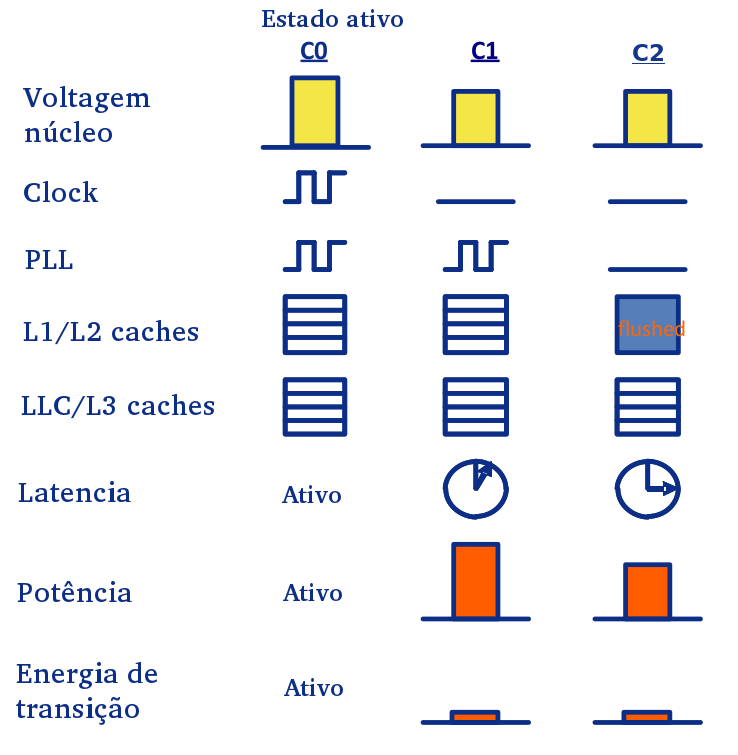
\includegraphics[width=\columnwidth]{intro/figures/c_states.png}
	\caption{C states}
\end{subfigure}%
~
\begin{subfigure}[t]{0.5\textwidth}
	\centering
	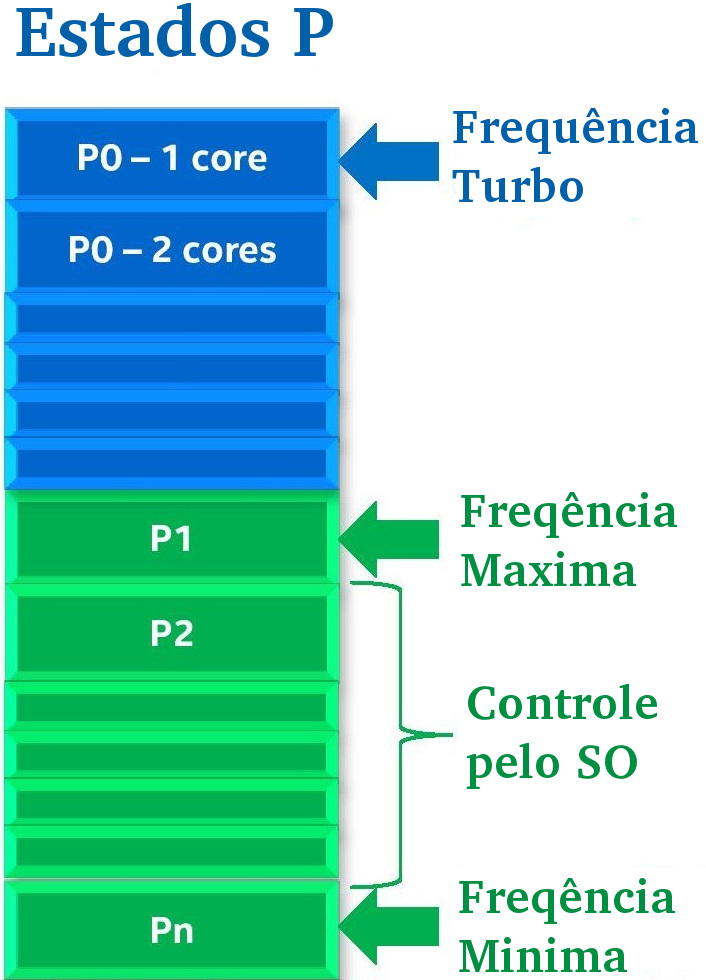
\includegraphics[width=\columnwidth]{intro/figures/p_states.jpg}
	\caption{States P}
\end{subfigure}
\caption {Illustration of states C and P} {Altered image from \protect \url {https://www.thomas-krenn.com/en/wiki/Processor_P-states_and_C-states}}
\label{fig:p_state}
\end{figure}


% Are states C and P orthogonal, do they operate independently?

For this management, the operating system provides in the user space a way to control the frequency. This work used an operating system that has Linux as its core.

Linux is compatible with several modern architectures and is widely used in servers, smartphones and supercomputers. It was based on the UNIX system which has the philosophy of treating everything on the system as a file, including settings and input and output devices, such as keyboard, mouse and hard drive. Another important feature is that it is modular and parts of the system can be loaded or removed during execution.

On Linux there are several frequency management options \cite {Brown2005ACPILinux}. The main ones are acpi-cpufreq, Intel P-state, AMD powernow. In this work, acpi-cpufreq is used, which is standard and allows direct control of frequency through system files. Acpi-cpufreq is a Linux module that uses implemented policies that dynamically decide the frequency to be used. Some of these policies are:

\begin{itemize}
\item Performance - configured as often as possible
\item Powersave - configured as low as possible
\item Userspace - the user chooses the frequency to be used
\item Ondemand - controls the frequency depending on the processor load. When the load increases the frequency also increases accordingly.
\item Conservative - similar to Ondemand but more smoothly, the frequency increase is continuous instead of jumping.
\end{itemize}

\section{Power consumption monitoring} \label{sec:power_consumption_monitoring}
The Running Average Power Limit (RAPL) and Intelligent Platform Management Interface (IPMI) interfaces were used to measure the power consumed. described in \cite{IPMI2013ConfigurationGuide}.

\subsection{IPMI}
IPMI \cite{IPMI2013ConfigurationGuide} is a set of specifications for autonomous subsystems that provides processor, firmware and operating system independent management and monitoring. The use of IPMI allows system administrators to avoid having to travel to the server location, which is often far away, to perform their tasks. Also, servers are located in places with low temperature and with a lot of noise due to the ventilation system, and one should avoid spending too much time in these places. With remote management, it is possible to turn the system on and off, remotely access the (BIOS) and reinstall the system in case of any serious failure.

\begin{figure}[H]
\centering
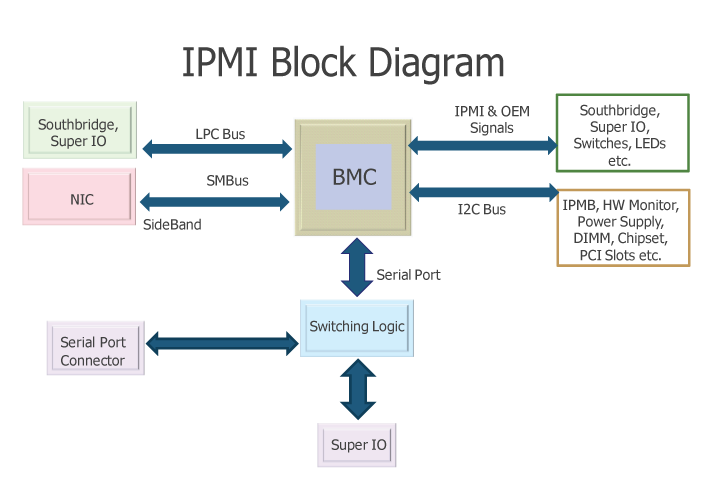
\includegraphics[height = 7.5cm] {intro/figures/IPMI-Block-Diagram.png}
\caption{IMPI diagram} {Image taken from \protect \url {https://pt.wikipedia.org/wiki/Intelligent_Platform_Management_Interface}, the main components of IPMI and how they communicate are shown}
\label{fig:IPMI}
\end{figure}

Access to the IPMI network can be done using the HTTP protocol or a tool made available by the manufacturer (ipmitool), which also performs access via the network. It is also used to monitor the status of the platform with a set of sensors coupled with system temperatures, voltages, fans and power supplies.

\subsection{RAPL}

Modern Intel microprocessors, based on the SandyBridge architecture, include the RAPL \cite {Rotem2012Power-managementBridge, Hahnel2012RAPL, Hackenberg2015AnProcessor} interface designed to limit the use of energy on a chip while ensuring maximum performance. This interface supports energy measurement capabilities through an integrated circuit that estimates energy use based on a model driven by architectural event counters for all components. It also provides temperature readings and current leak models. Estimates are made available in model-specific registers (MSR), updated in milliseconds. The energy estimates offered by RAPL were validated by Intel, which showed excellent results.

\section{Case-Study architecture} \label{sec:casestudyarchitecture}
The experiments were executed in one computer node equipped with two Intel Xeon E5-2698 v3 processors with sixteen cores each and two hardware threads for each core. 
The overall view of the architecture is shown in \cref{fig:architecture}.
The maximum non-turbo frequency was 2.3 GHz, and the total physical memory of the node was 128 GB (8 $\times$ 16 GB). Turbo frequency and hardware multi-threading were disabled during all experiments. The operating system used was Linux CentOS 6.5, kernel 4.16. 

\begin{figure}[H]
\centering
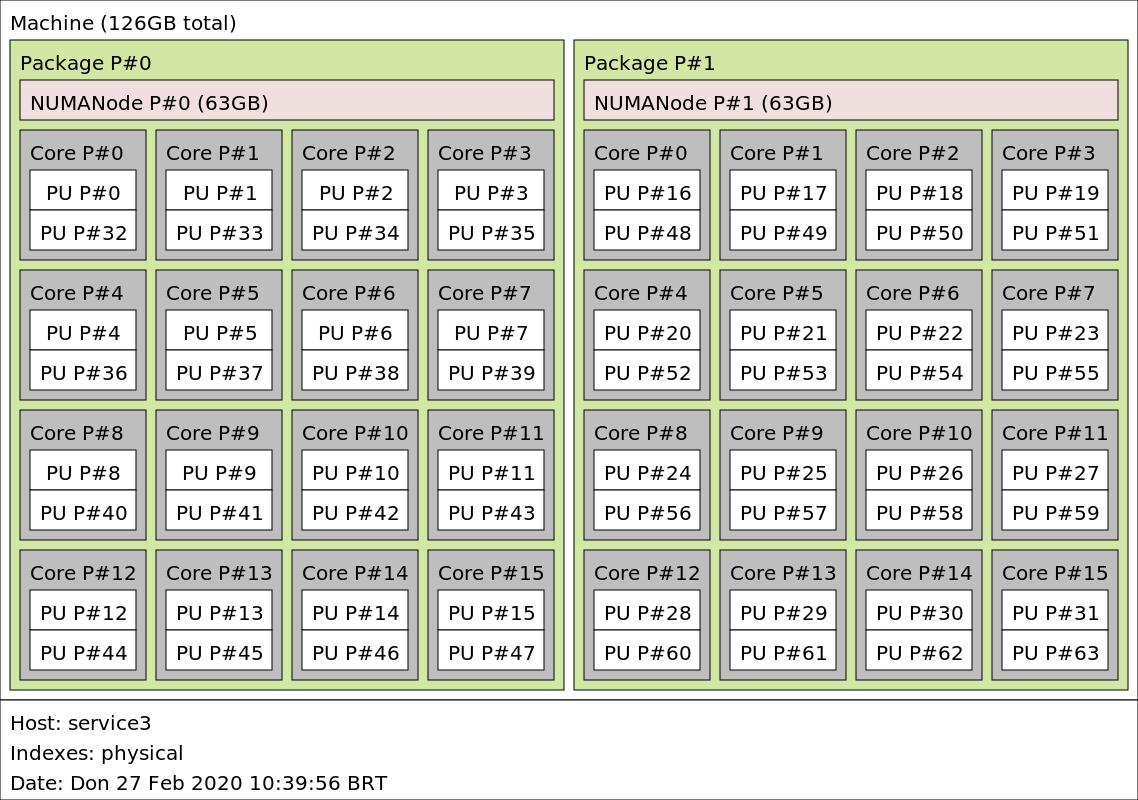
\includegraphics[width=\columnwidth]{models/figures/architecture.png}
\caption{Node architecture (the image was made with the lstop application).}
\label{fig:architecture}
\end{figure}

The Linux kernel has many different policies for power management, depending on the driver. In the default driver, the acpi-cpufreq, the options are Powersave, Performance, Ondemand, Conservative, and Userspace. Each governor has a policy on how the frequency is selected. In this investigation, the frequency control was performed using the Userspace governor, which allows the user or any userspace program to set the CPU to a specific frequency. The core control was accomplished by modifying the appropriate system files with the default CPU-hotplug driver.

The architecture was equipped with the intelligent platform management interface (IPMI), a set of interfaces allowing out-of-band management of computer systems and platform-status monitoring via the local network~\cite{Schwenkler2006IntelligentInterface}. It can monitor variables and resources, such as the system's temperature, voltage, fans, and power supplies, with independent sensors attached to the hardware.

\section{Case-Study applications} \label{sec:casestudyapplication}
The applications blackscholes, bodytrack, canneal, dedup, fluidanimate, freqmine, raytrace, swaptions, vips and x264 from the PARSEC \url{https://parsec.cs.princeton.edu/download.htm} (accessed on 20 February  2020) parallel benchmark suite, version 3.0~\cite{Bienia2008TheSuite}, OpenMC \cite{Romano2015OpenMC:Development} and LINPACK (HPL) \cite{Dongarra1988TheExplanation}, were chosen as case studies. The PARSEC benchmark focused on emerging workloads and was designed to represent the next-generation shared-memory programs for chip-multiprocessors. It covers an ample range of areas, such as financial analysis, computer vision, engineering, enterprise storage, animation, similarity search, data mining, machine learning, and media processing. The OpenMC and the LINPACK are two classic HPC programs.

%The other two experiments use applications Raytrace~\cite{Bienia2008} and OpenMC~\cite{Romano2015OpenMC:Development}. Raytrace is an application addressed on rendering photorealistic scenes. It is available on the PARSEC Benchmark suite, version 2.0. The PARSEC benchmark, focused on emerging workloads, represents the next-generation shared-memory programs for chip multiprocessors. It covers a wide range of areas such as financial analysis, computer vision, engineering, enterprise storage, animation, similarity search, data mining, machine learning, and media~processing.
%
%\textls[-20]{{OpenMC is an application that implements the Monte-Carlo method to simulate the transport of neutrons and photons. It is a classic program aimed at high-performance computing.}}

